\subsection{Overview of the Treatment Plant}

The \ac{WWTP} located at Moratuwa/Ratmalana was chosen as the study location for this study. It was established in 2013 under the \ac{NWSDB} of Sri Lanka. It has been designed with a total capacity of 17,000 \unit{m^3}/day. Four pumping stations located at Badowita, Ratmalana, and Thelawala supply wastewater from 5,700 domestic and 239 industrial connections directly to this plant, and 510 \unit{m^3}/day (3\% of the total capacity) is supplied by gully bowsers.

The Moratuwa/Ratmalana Treatment Plant is a biological treatment plant that uses the activated sludge method to treat wastewater. The biological basin has been designed using the reverse A2O system, and the Moratuwa/Ratmalana \ac{WWTP} is the first-ever reverse A2O plant in Sri Lanka \cite{Danushika2016}. There are primary, secondary, and tertiary treatment processes at this premises. 

\begin{figure}[H]
\centering
\includegraphics[width=0.756\linewidth]{connection_network_map.png}
\caption{Connection network map; source: \ac{NWSDB}}
\label{fig:connection_network_map}
\end{figure}



\subsubsection{Primary Treatment}
Wastewater arrived at the collecting chamber by gravity from four pumping stations and from the septic sludge receiver, which unloaded the gully. Collected wastewater in the inlet chamber goes through the coarse screen that has free slots of 40 mm between the bars to remove large matter from the wastewater. After the coarse screening, the flow arrives at the inlet well and is pumped to the fine screen by an inlet pumping station equipped with three submersible pumps. Pumped wastewater goes through a fine screen that has free slots of 3 mm between the bars to remove small particles. The screened water arrives at the grit traps to settle and remove the sand and heavy particles. Pretreated water is collected in the collecting chamber, and there is a bypass to control the overflow higher than the design flow. Before the secondary treatment, the split box is fixed to divide the flow into two streams.

\subsubsection{Secondary Treatment/Biological Treatment}
Biological treatment started in the denitrification basin, and 60\% of the influent flow arrived at the basin that was divided by the split box, mixed with the return-activated sludge recirculated from the clarifiers. There is a low dissolved oxygen content, but the oxygen that is bound with nitrogen as nitrate is available in the flow. Therefore, these denitrification basins have anoxic conditions, and denitrification occurs under these conditions. For better denitrification, it is necessary to keep the oxygen concentration in the basin below 0.5 \unit{mg/l}. There is a 2.8 \unit{hour} retention time in the anoxic basin. 

After denitrification, wastewater arrives at the anaerobic basin and is mixed with 40\% of the influent flow divided by the split box. Anaerobic basins do have a concentration of dissolved oxygen, and under this anaerobic condition, phosphorous-accumulating microorganisms store organic materials and release the phosphorous. The untreated influent that arrives from the split box ensures the availability of easily biodegradable organic matter. There is a 1.3 \unit{hour} retention time in the anaerobic basin.

After the anaerobic basin, wastewater arrives at the aerobic basin for nitrification. Here, microorganisms metabolize organic matter by consuming oxygen and releasing carbon dioxide and water. Microorganisms use organic matter and nutrients as an energy source for growth. In an anaerobic tank, nitrification is prominent under a dissolved oxygen concentration range of 1.5-2.0 \unit{mg/l} and occurs as per the following formula:
\begin{gather}
    \ce{NH4^+_{(aq)} + 2 O2_{(aq)} -> NO3^-_{(aq)}  + H2O_{(l)}  + 2 H^+_{(aq)}}
\end{gather}

The fine bubbler rubber membrane diffusers are installed at the bottom of the basin to distribute the air, and the oxygen concentration is controlled by oxygen meters. All three basins are equipped with submersible mixtures to obtain complete contact with the wastewater and the sludge and avoid settling the sludge. There is a 9.9 \unit{hour} retention time in the aerobic basin.

\begin{figure}[H]
\centering
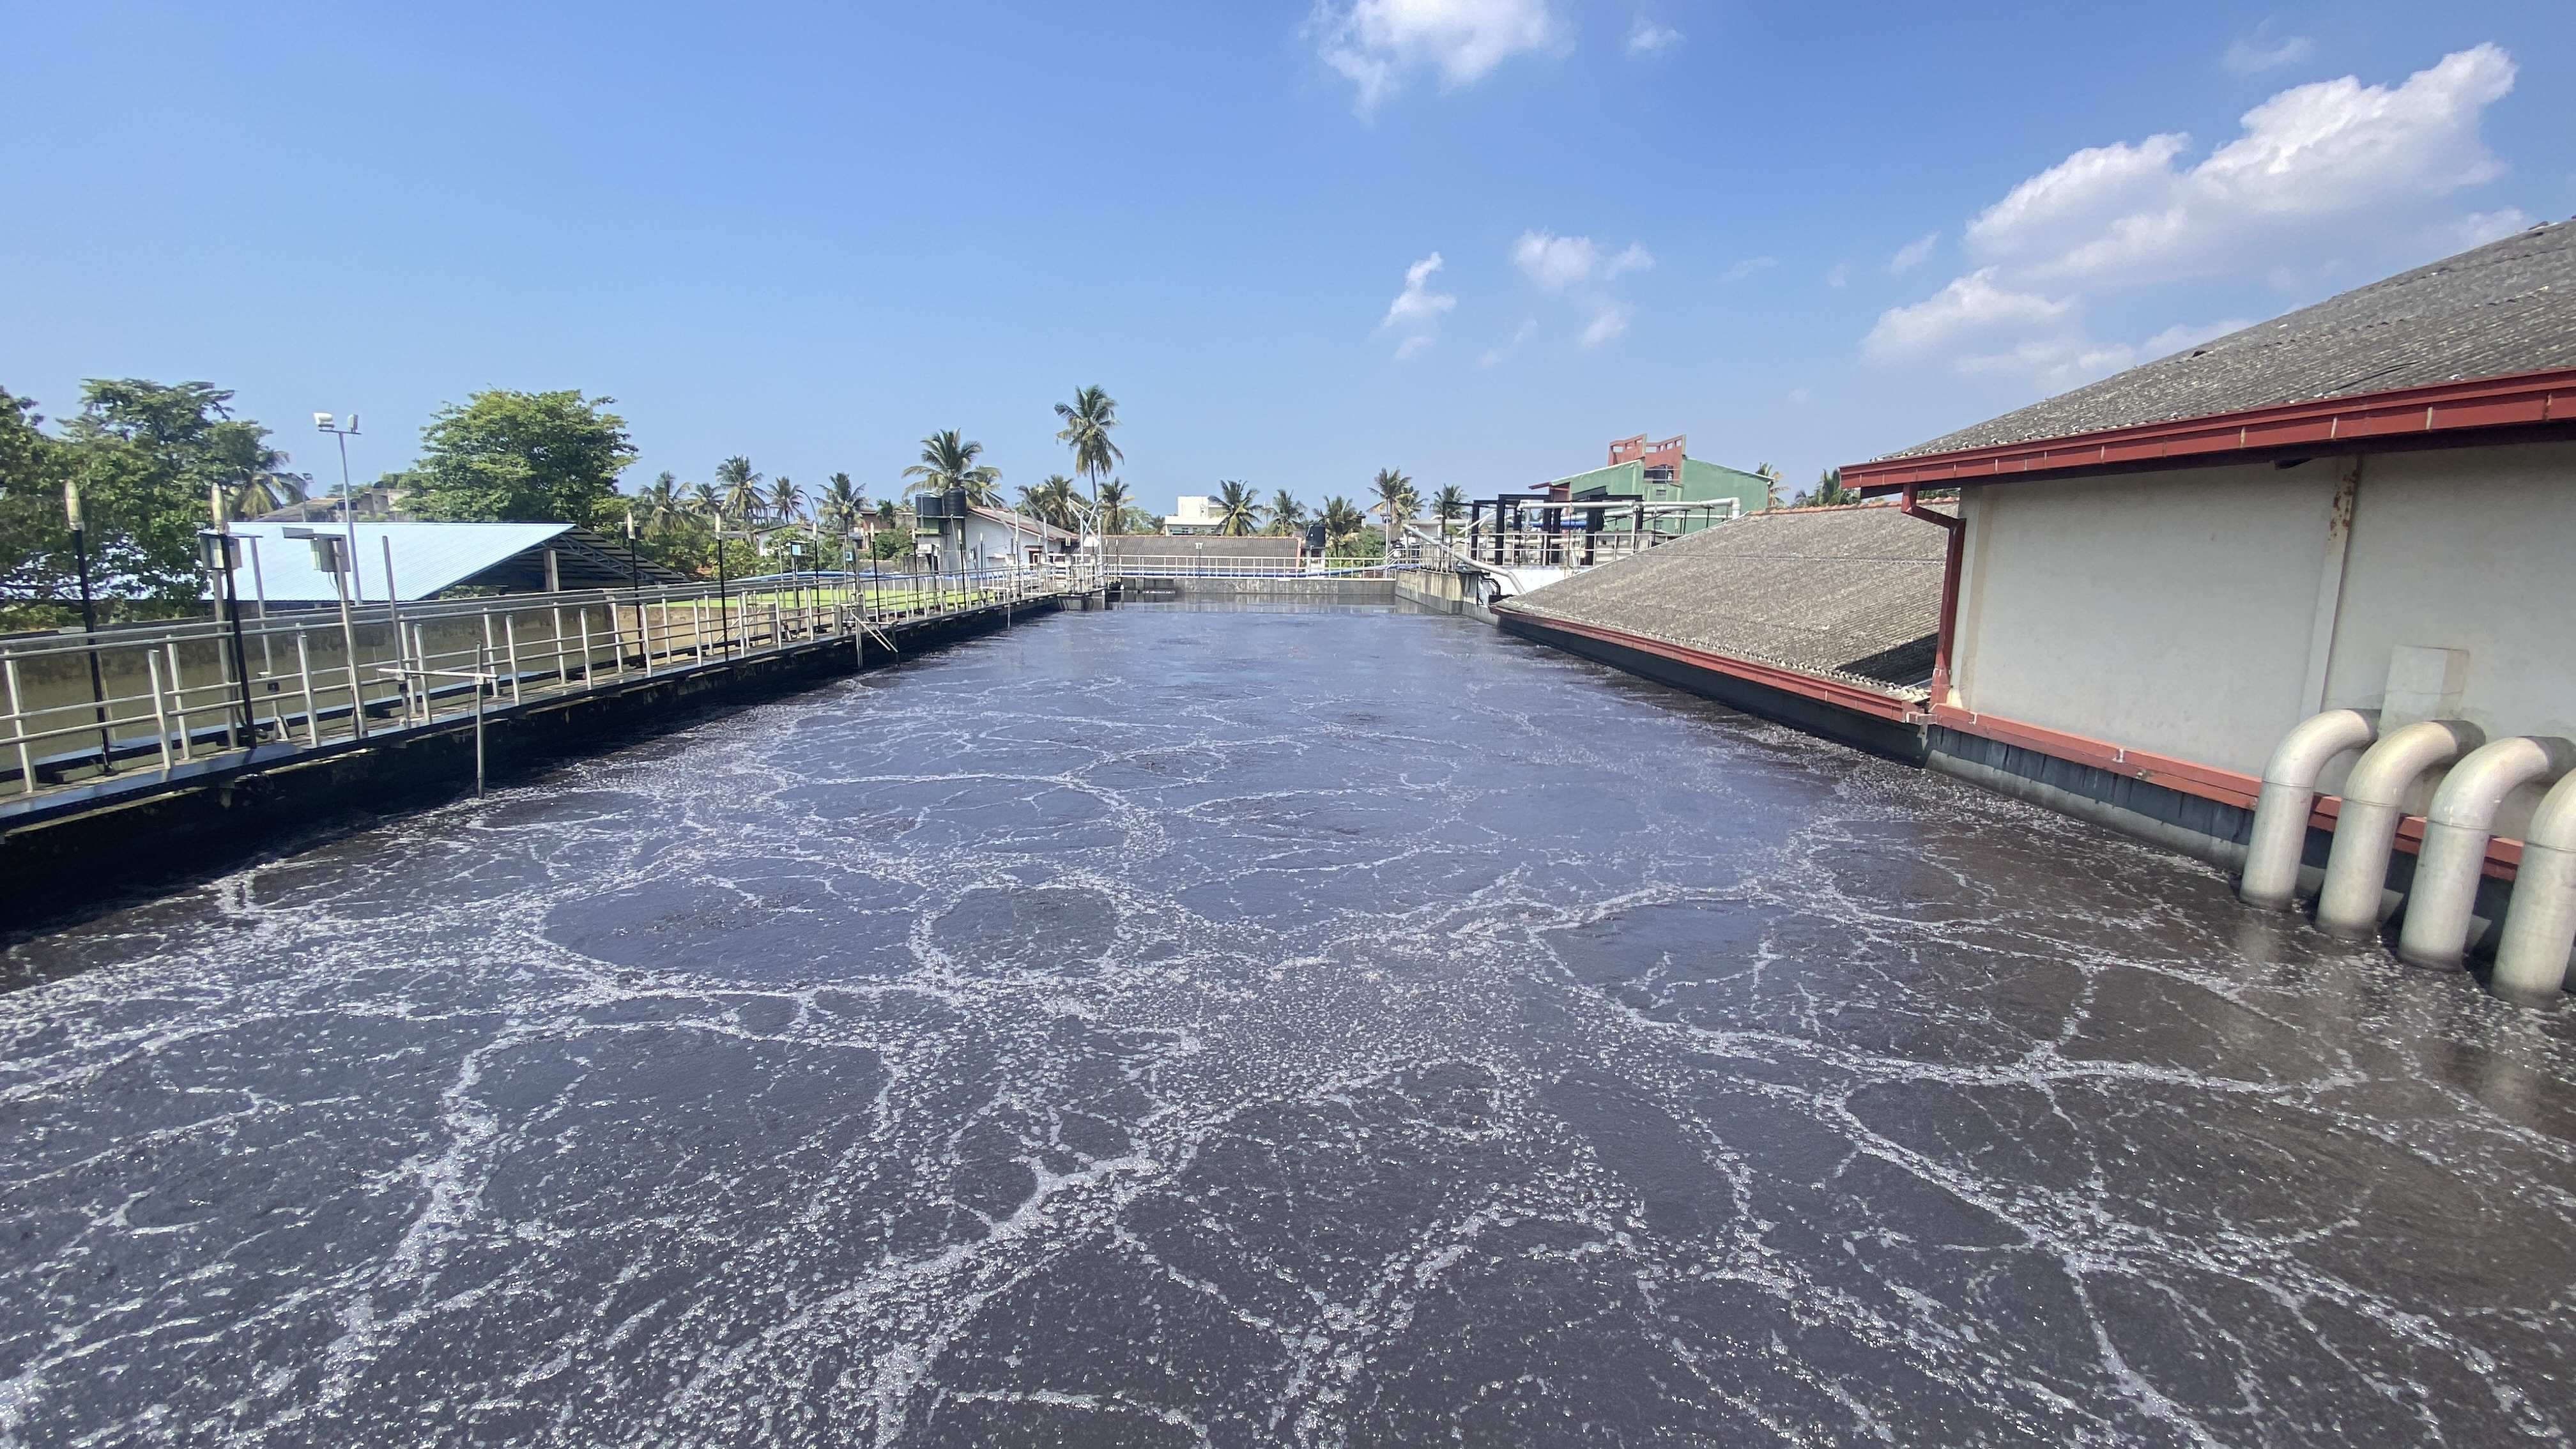
\includegraphics[width=0.98\linewidth]{material_and_methodology/Biological Treatment basins.JPG}
\caption{Biological treatment basins}
\label{fig:Biological_treatment_basins}
\end{figure}

After the biological treatment, the treated wastewater arrives at the sedimentation tank for clarification. In the sedimentation tank, gravitational forces separate the activated sludge flocks from the treated wastewater. The traveling bridge siphon scraper is installed at the sedimental tank to lift the sludge from the bottom of the sedimentation tank to a longitudinal sludge channel by siphon action. Once the biological treatment is completed, the treated wastewater is led to the treated water channel. There is a 6.9 \unit{hour} retention flow through the clarifiers.

\begin{figure}[H]
\centering
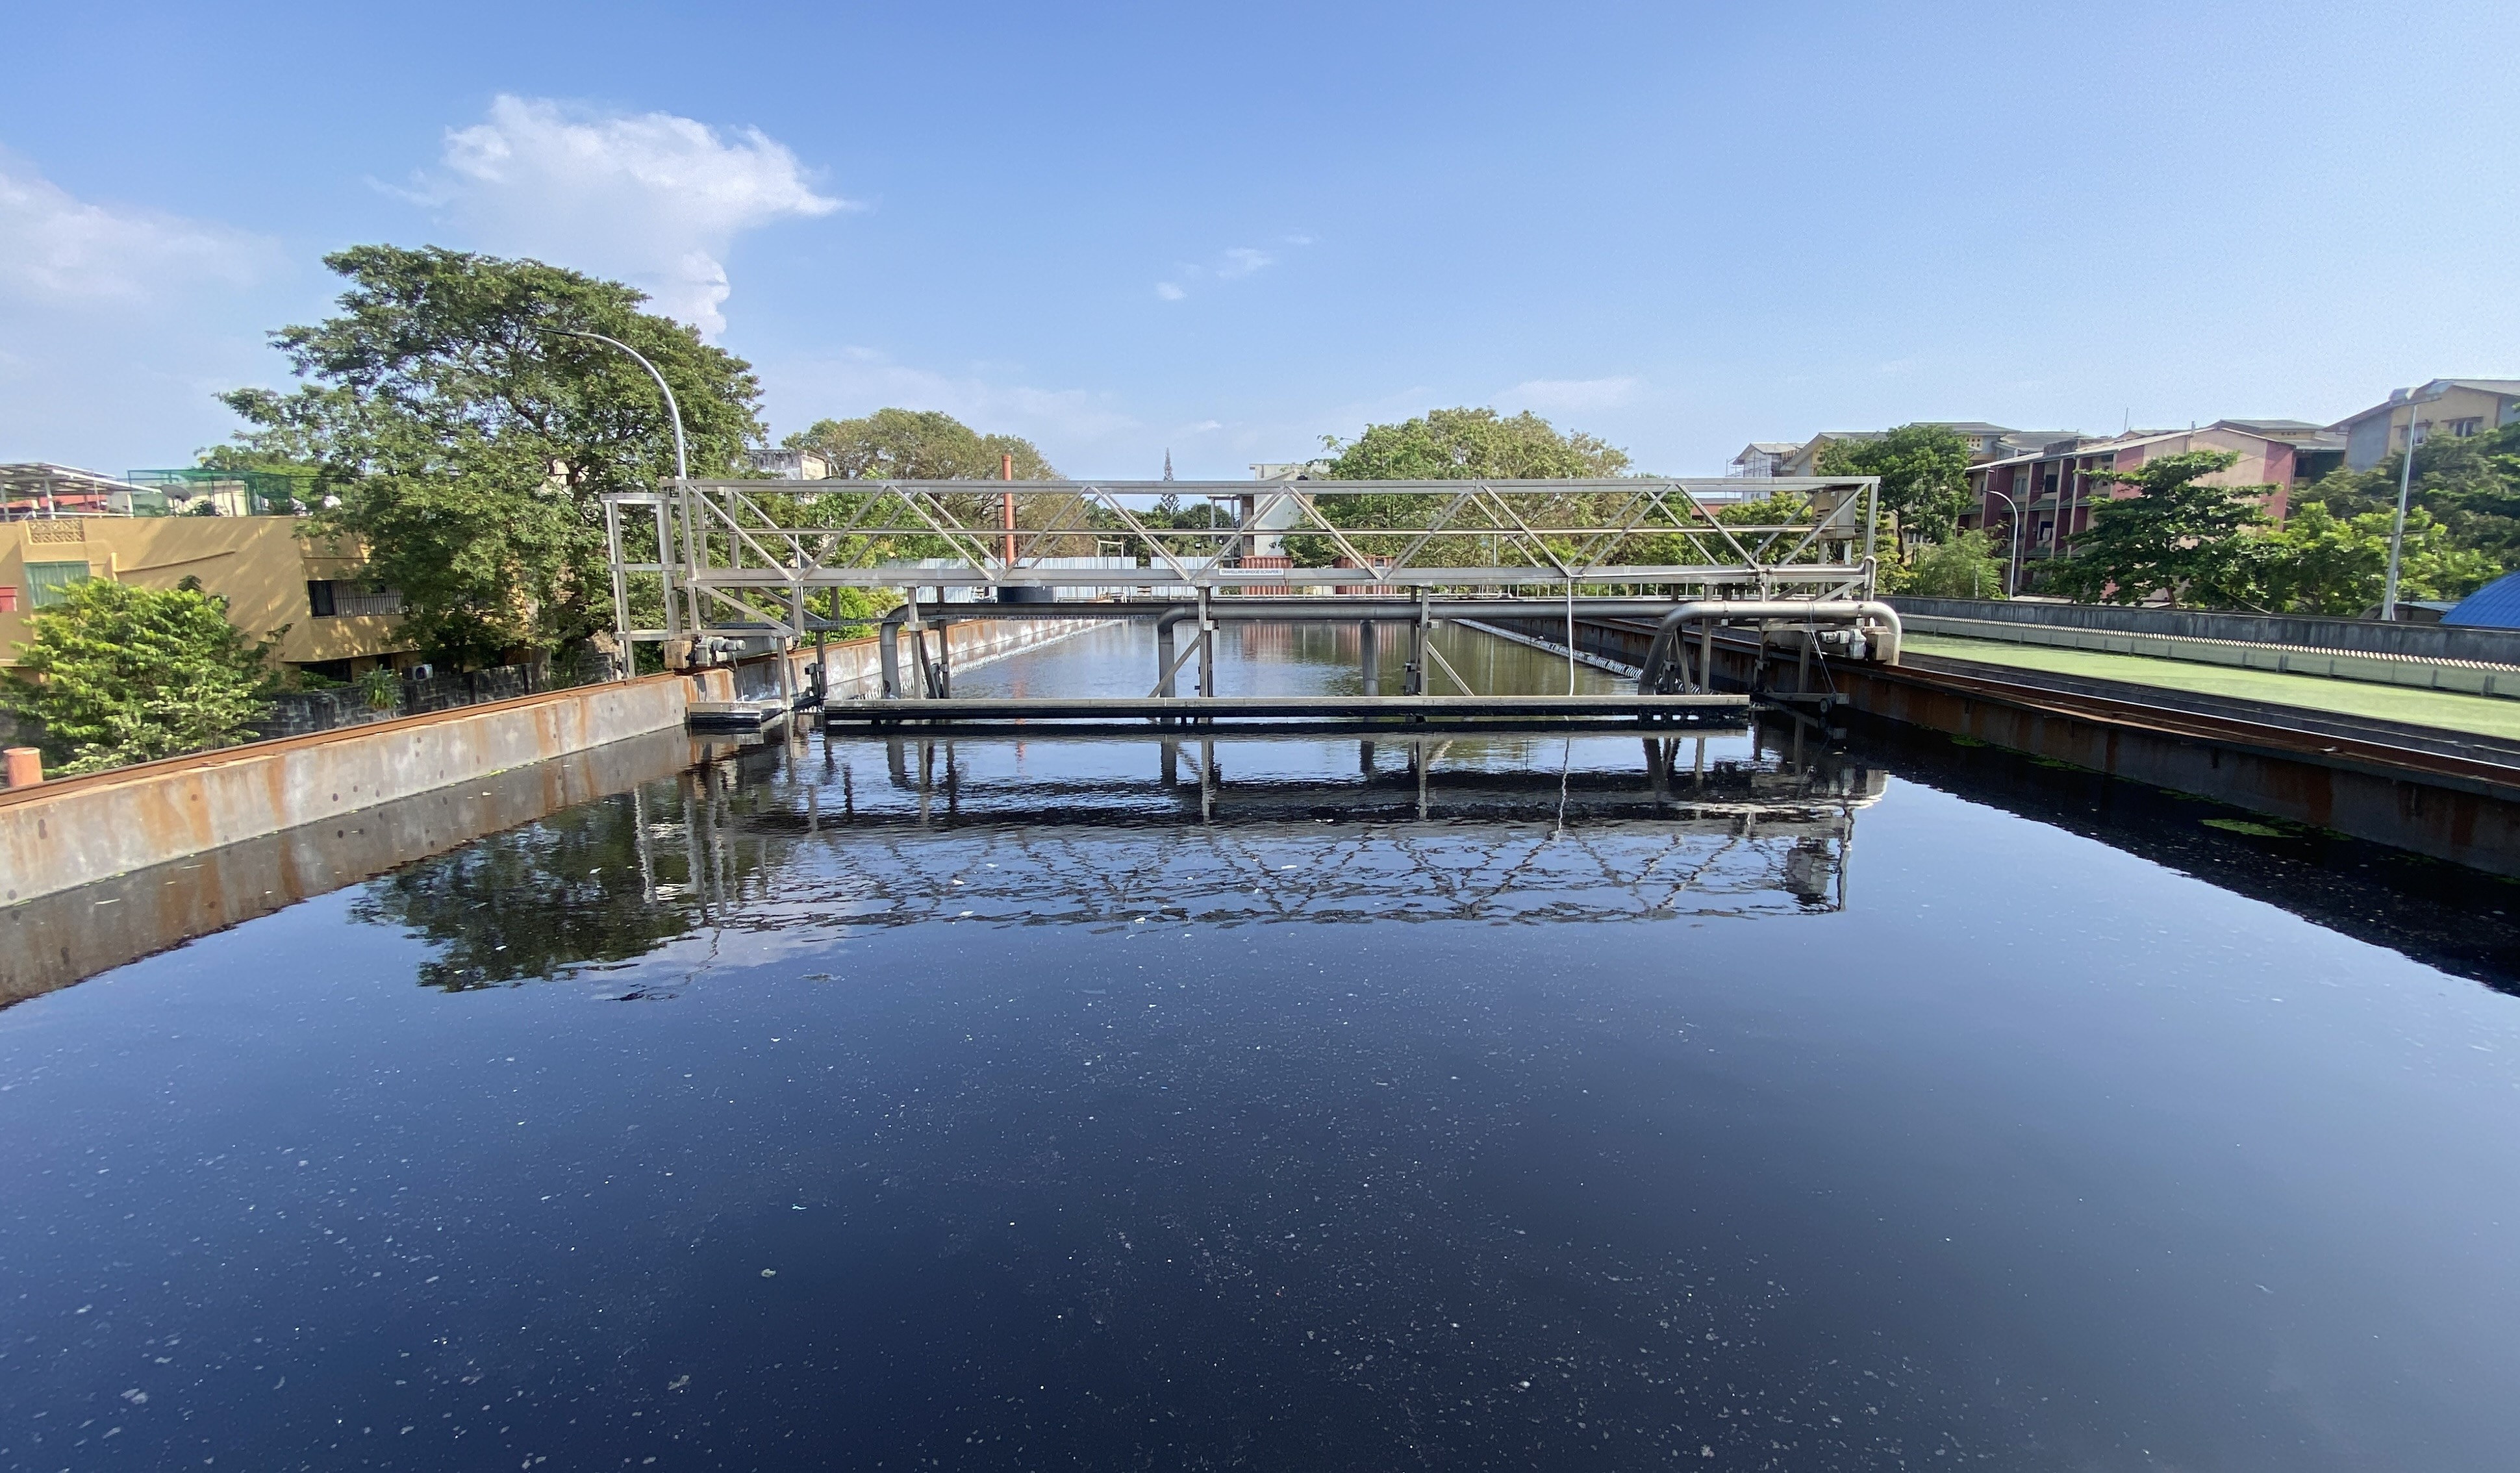
\includegraphics[width=0.98\linewidth]{material_and_methodology/Sedimentation basin.jpg}
\caption{Sedimentation tank}
\label{fig:Sedimentation_tank}
\end{figure}
\subsubsection{Tertiary Treatment/Chemical Treatment}
Sodium hypochlorite is used in the chlorination unit to disinfect the treated wastewater. Hypochlorite is dosed at the outlet flow in cases of epidemic diseases in circulation. The treated wastewater was discharged by a short sea outfall in the Angulana area.  

\subsubsection{Compost Filter}
Ventilation Air collected from septic sludge handling, screen washers, screening containers, sand separators, and grit containers is transported by a fan to a compost filter for odor reduction. Compost filters are filled with small pieces of coconut husk to grow the microorganisms. The treated wastewater is sprayed into the tank to protect the coconut husk's moisture content and ensure the microorganisms' growth. 

\begin{figure}[H]
\centering
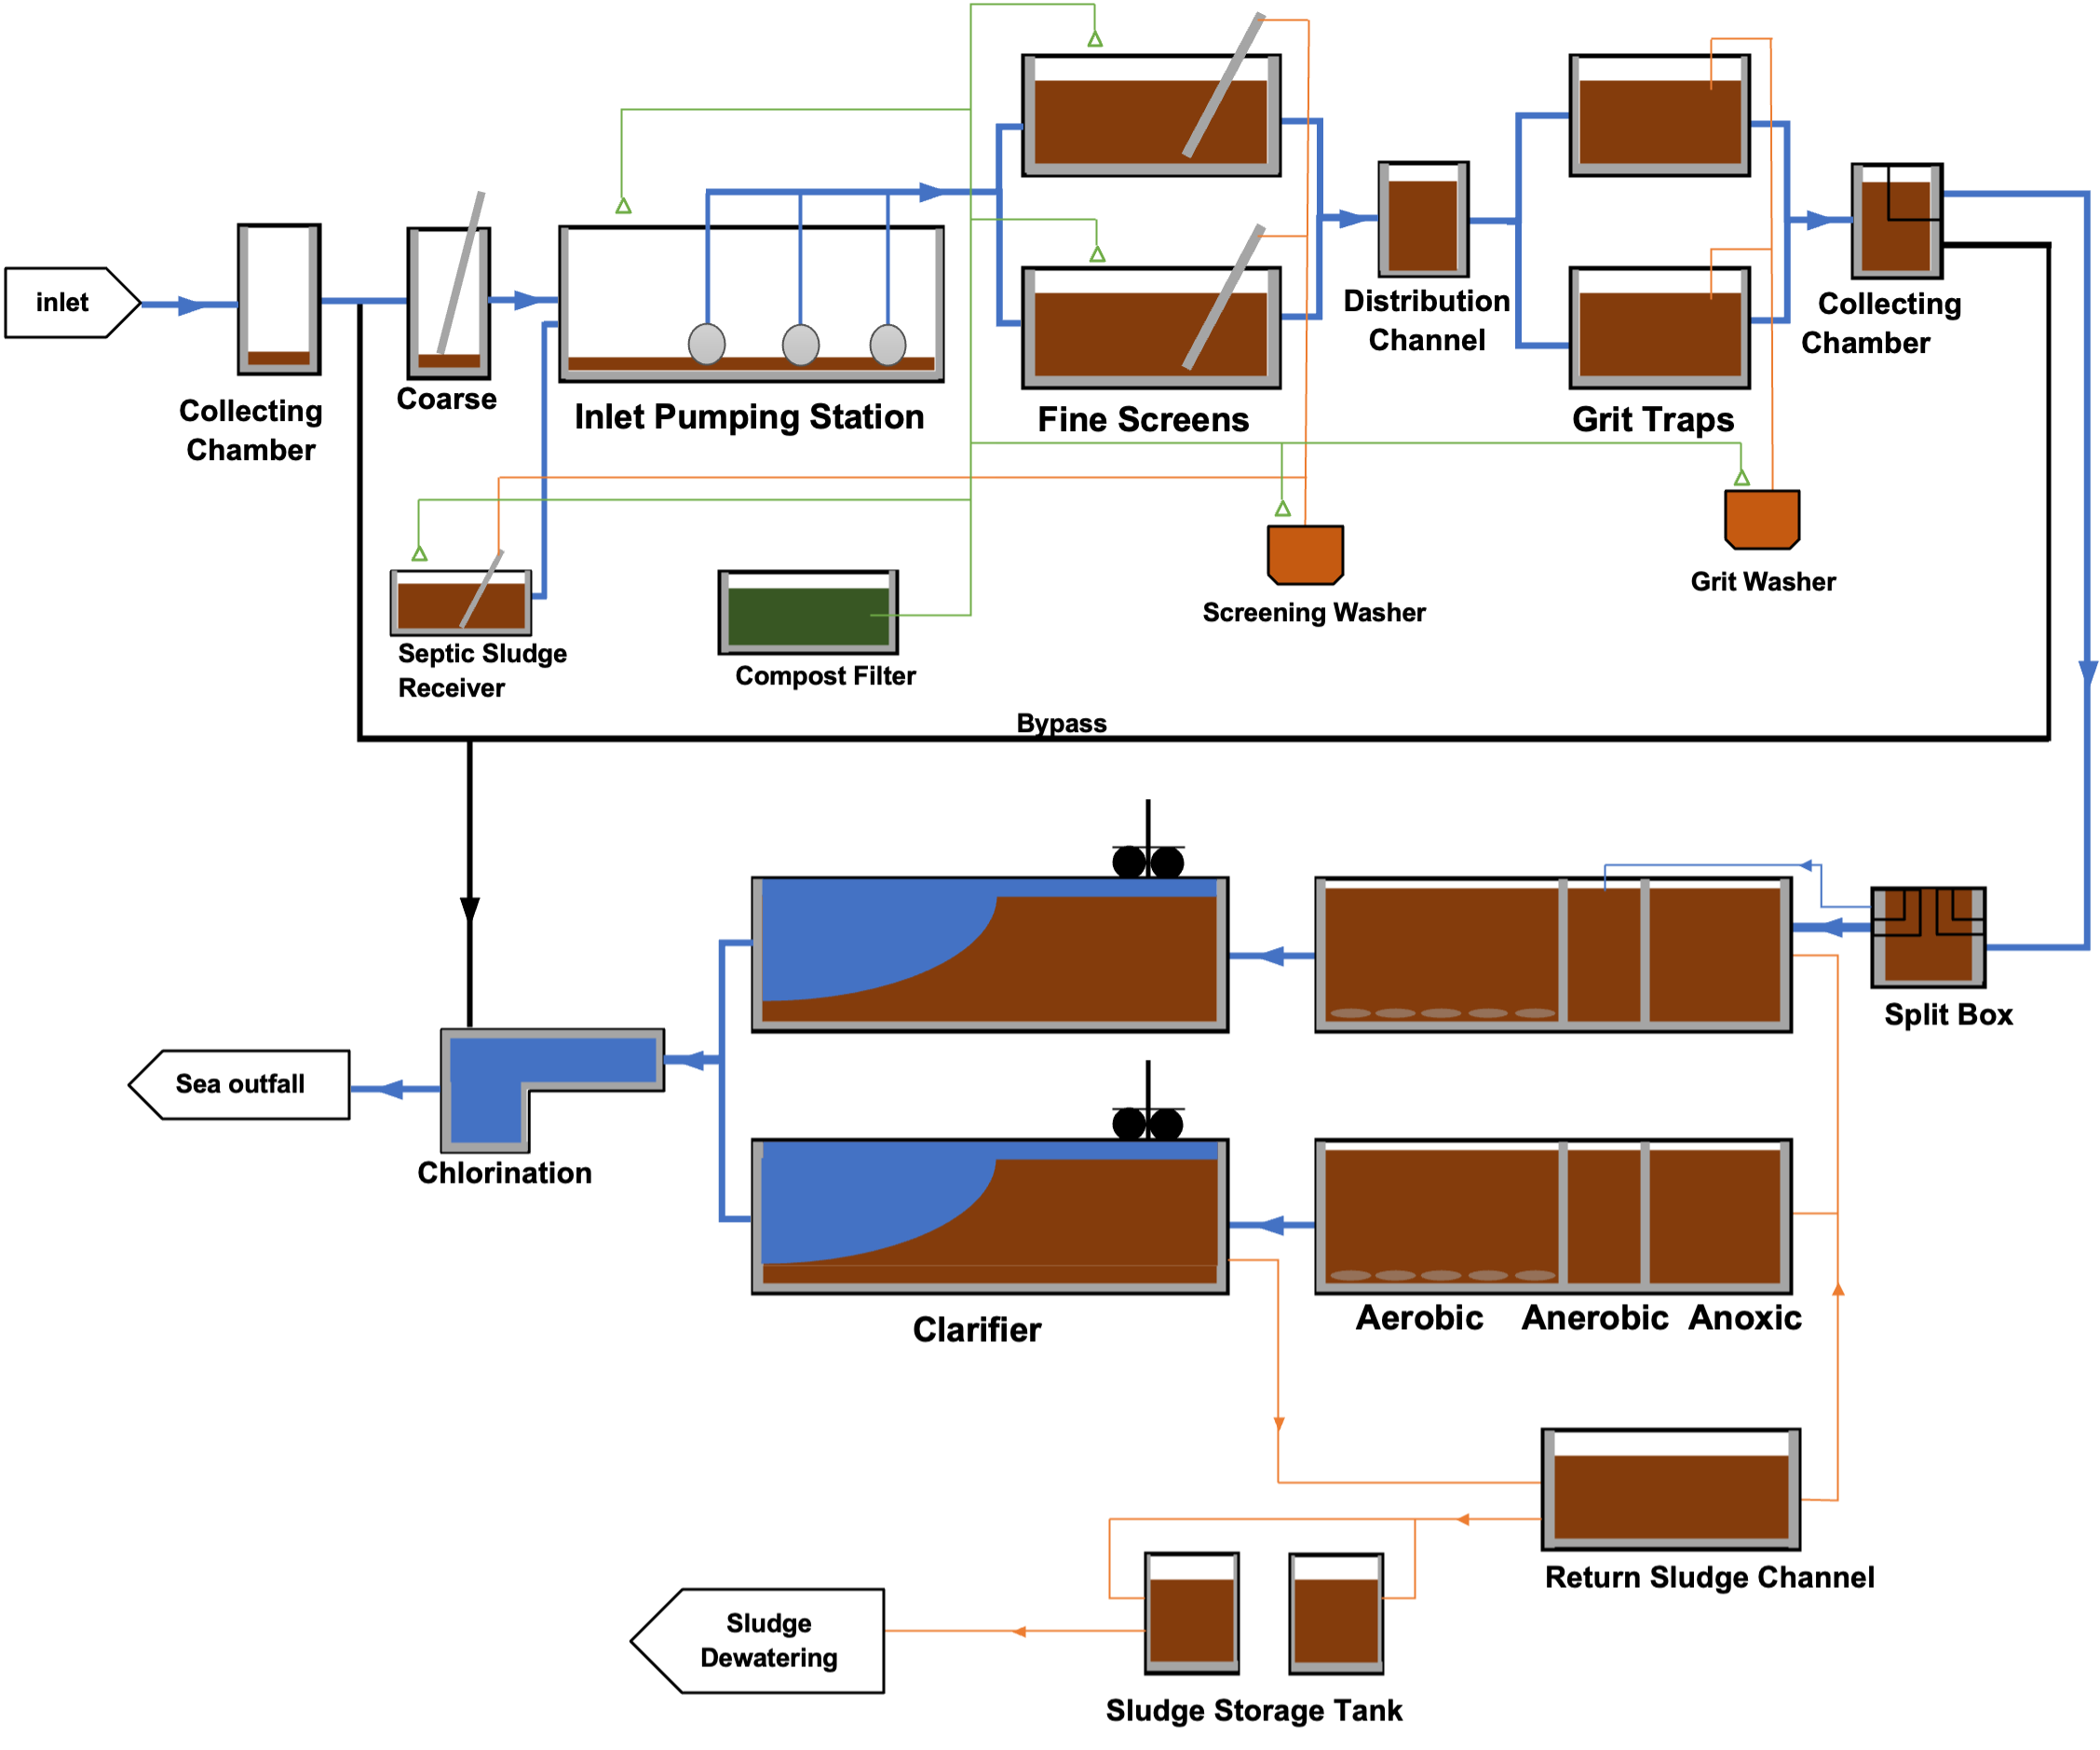
\includegraphics[width=1\linewidth]{material_and_methodology/diagram_of_treatment_plant.png}
\caption{Schematic Diagram of the Wastewater Treatment Plant}
\label{fig:treatment_plant}
\end{figure}

\subsubsection{Sludge Treatment}
If the suspended solid concentration in the return sludge channel is higher than the limit, the excess sludge is withdrawn from the return sludge flow. The sludge flow arrives at either one of two sludge storage tanks. The sludge storage tanks have submersible mixers to avoid sedimentation during dewatering, and from the storage tank, the sludge is pumped to the belt filter press for dewatering. Before dewatering sludge, the digested sludge is typically treated to create flocs that can be easily filtered \cite{Chen2002}. Therefore, a polymer solution (cationic polyacrylamide) is dosed into the sludge flow. Belt filter presses typically include two or, in some instances, three filtering belts that converge to create a closed envelope shape. The flocculated sludge is first dewatered by gravity and then compressed between two belts. Filtration takes place in the gravity drainage zone without applying pressure to the sludge. The sludge solids percentage is typically between 6\% and 10\% after water drainage. Subsequently, as pressure rises, water trapped inside and between sludge particles is expelled \cite{Mamais2009}. The sludge flow to the belt press is measured with a flow meter, and the dewatered sludge is carried from a belt filter press to the truck using a screw conveyor and transported to the drying bed.

\begin{figure}[H]
\centering
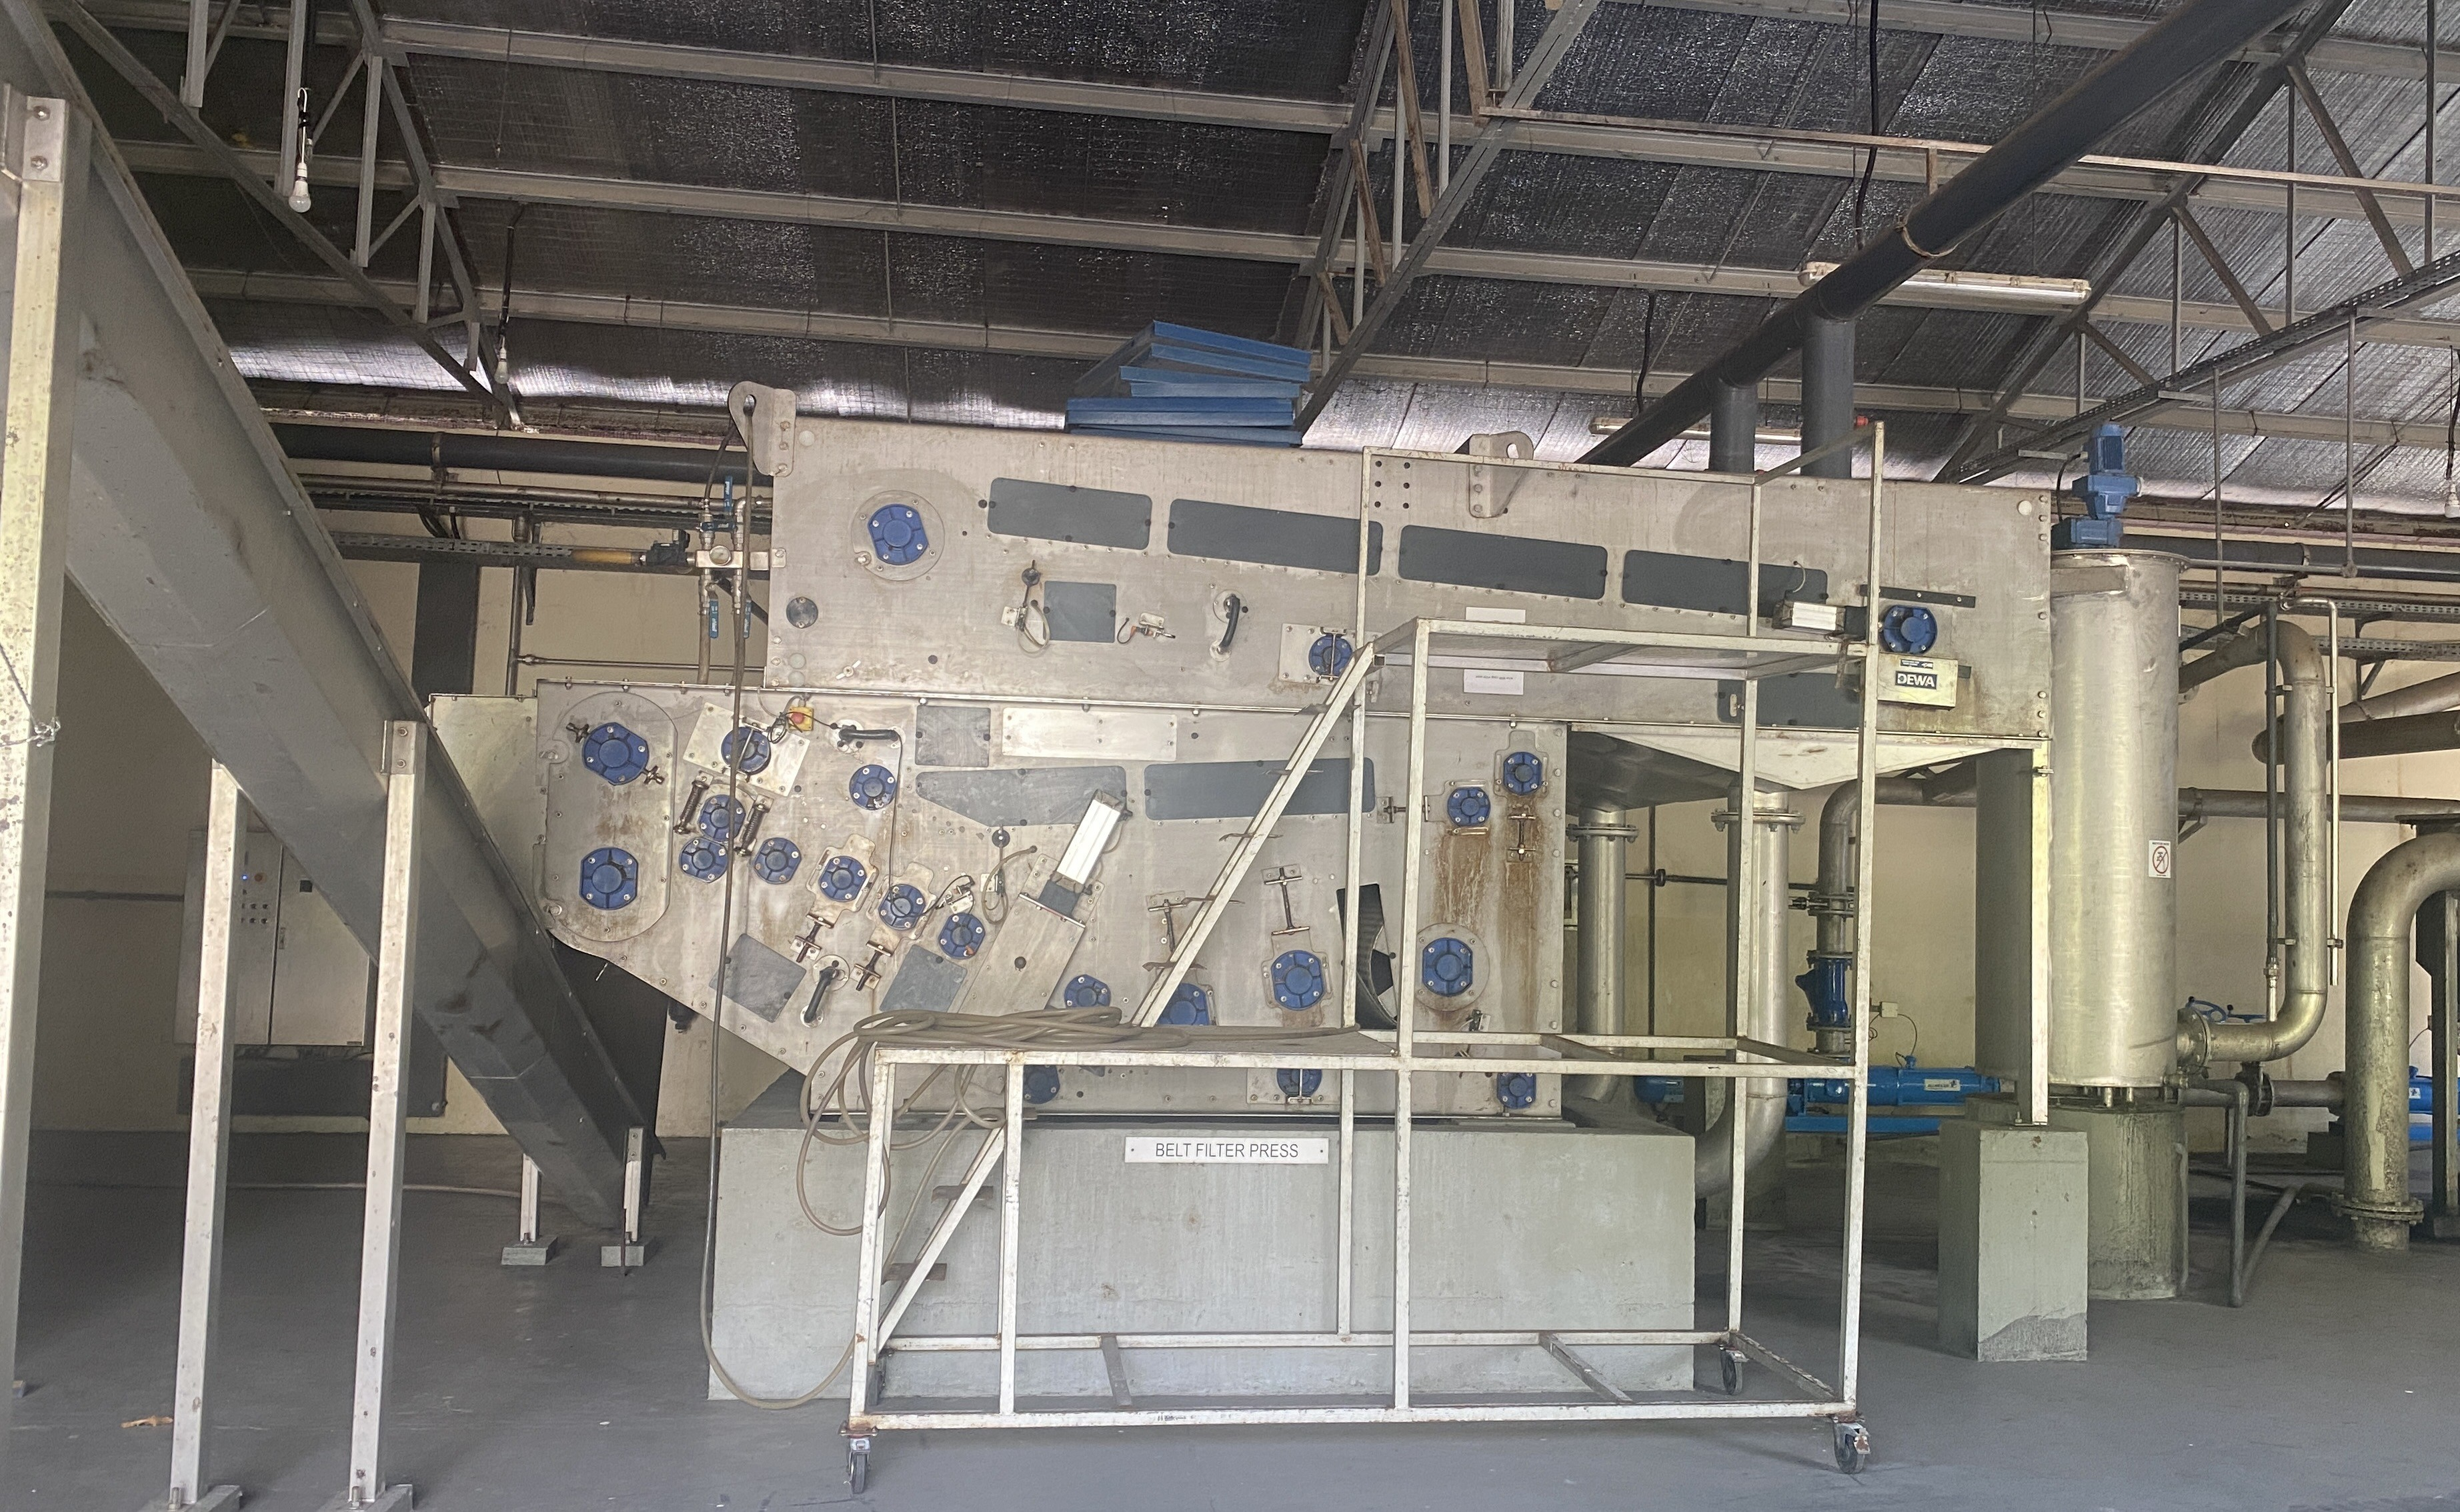
\includegraphics[width=1\linewidth]{material_and_methodology/Belt press.jpg}
\caption{Belt Filter Press}
\label{fig:Belt_filter_press}
\end{figure}

\begin{figure}[H]
\centering
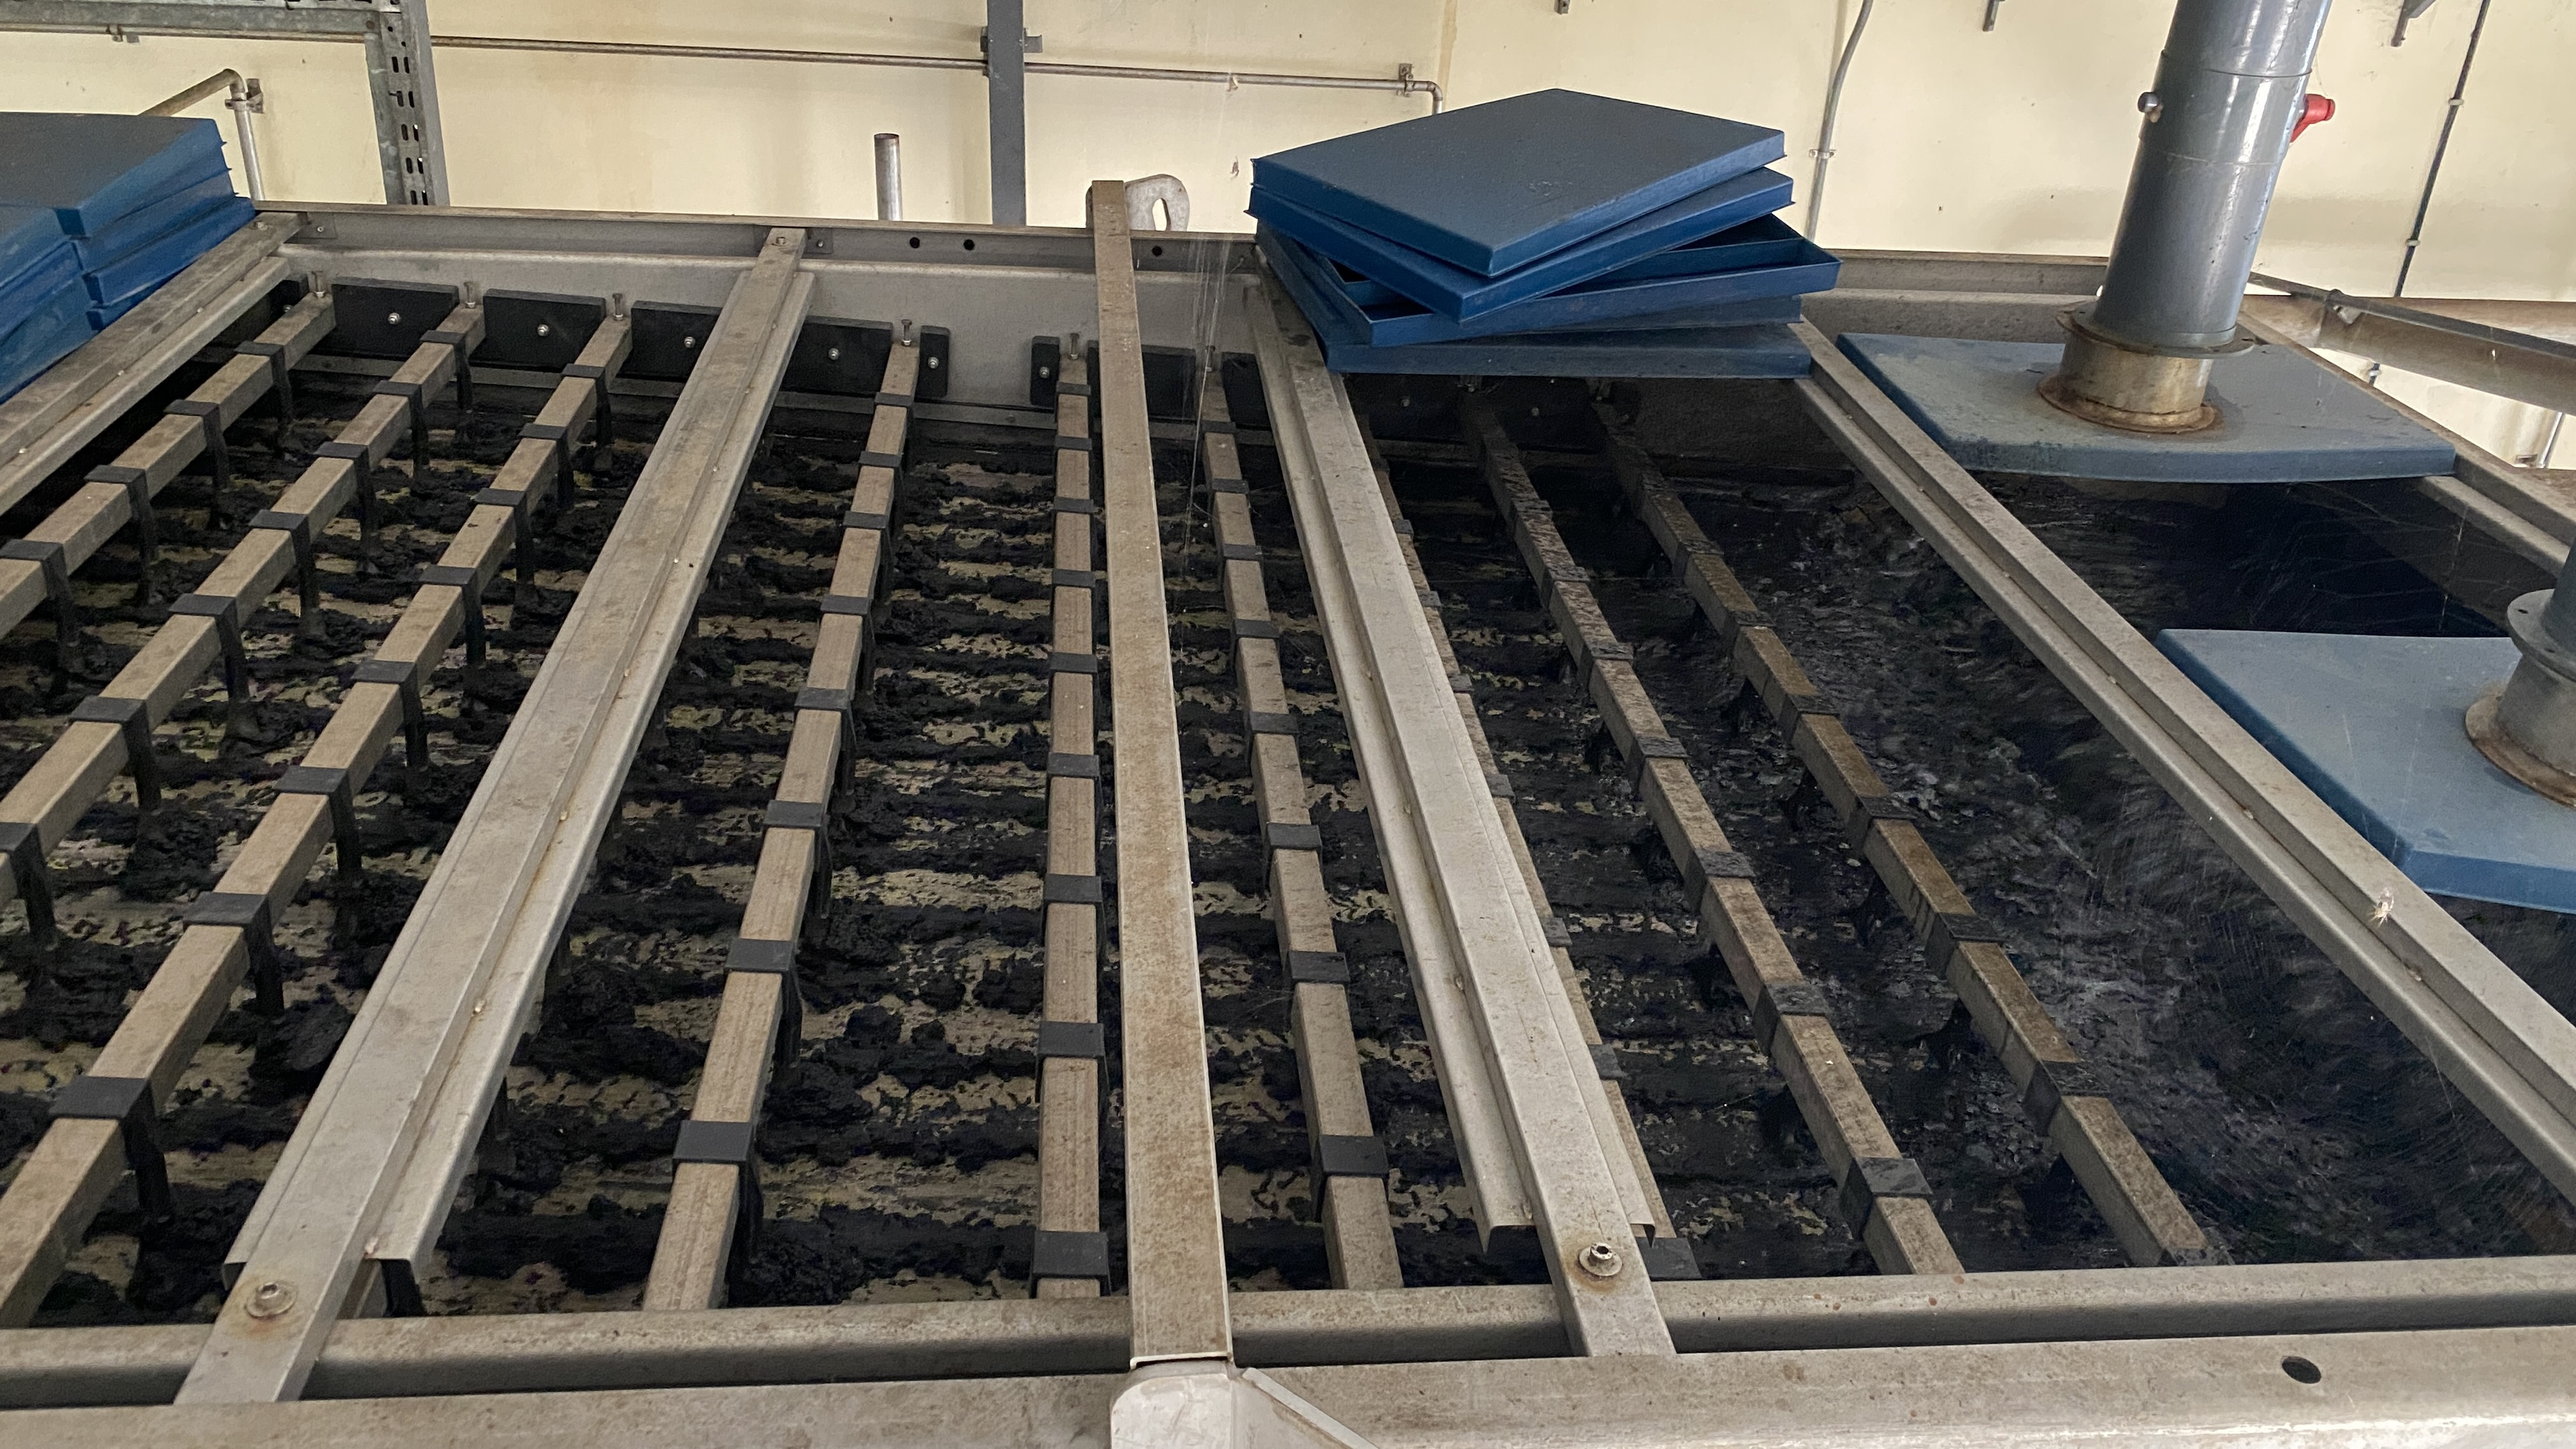
\includegraphics[width=0.98\linewidth]{material_and_methodology/Beltpress feeding area.JPG}
\caption{Belt Filter Press feeding area}
\label{fig:Beltpress_Feeding_area}
\end{figure}

There are 5 large and 10 small fans equipped at the drying bed that work 24 hours to decrease the inside humidity. There is a large fan that draws out the inside air. There is a rotary that activates hourly for thinning sludge.

\begin{figure}[H]
\centering
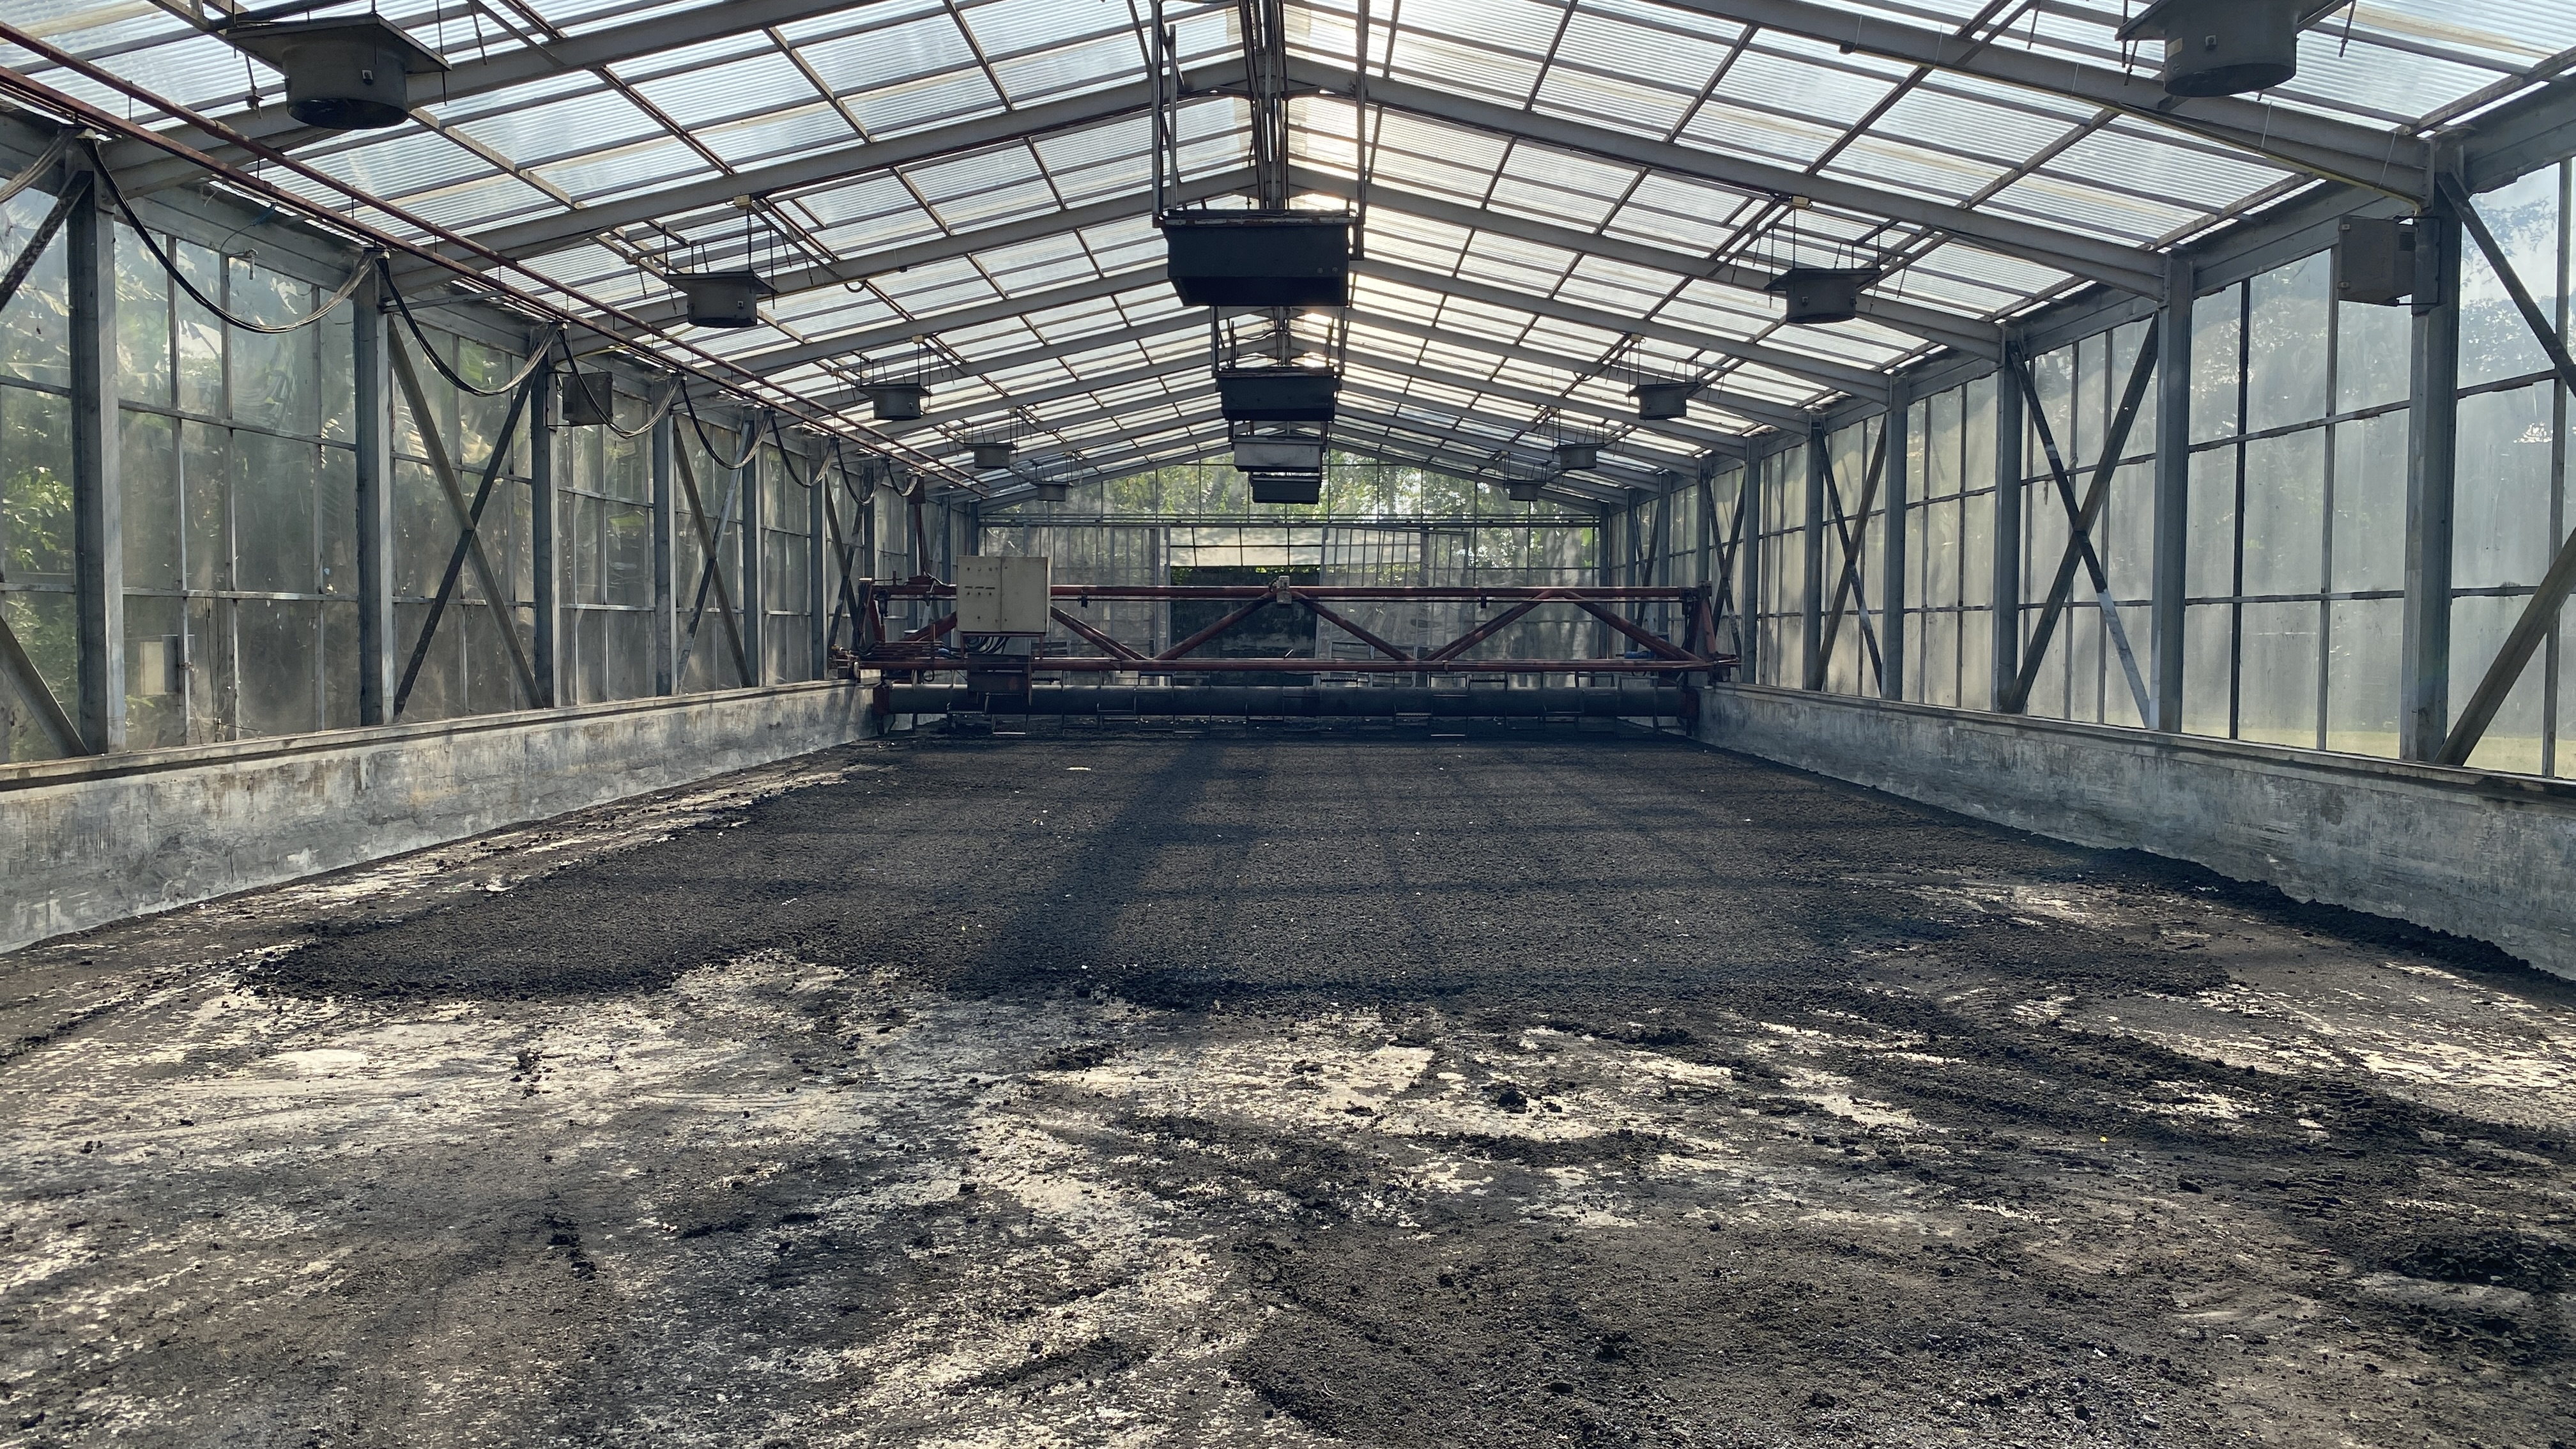
\includegraphics[width=0.98\linewidth]{material_and_methodology/Sludge Drying bed.jpg}


\caption{Sludge drying bed}
\label{fig:Sludge_Drying_Bed}
\end{figure}
